% Maerz 2015
% Autor: Mandy Vogel
% Tests 
\documentclass[xcolor={table}]{beamer}
\usetheme{Singapore}

%% \usepackage{listings}
\usepackage{linkimage}

\begin{document}

\title{Classical Tests}   
\author{Mandy Vogel} 
\date{\today}
%\logo{\includegraphics[scale=0.14]{PIC1}}

\begin{frame}
\titlepage
\end{frame}

\begin{frame}
\frametitle{Table of Contents}\tableofcontents
\end{frame}


\section{Exercises}
\subsection{dplyr/ggplot2}
\begin{frame}\frametitle{Exercises} 
  \begin{enumerate}
  \item load the data (file: session4data.rdata)
  \item make a new summary data frame (per subject and time) containing:
    \begin{itemize}
    \item the number of trials
    \item the number correct trials (absolute and relative)
    \item the mean TTime and the standard deviation of TTime
    \item the respective standard error of the mean
    \end{itemize}
  \item keep the information about Sex and Age\_PRETEST
  \item make a plot with time on the x-axis and TTime on the y-axis showing the means and the 95\% confidence intervals (\texttt{geom\_pointrange()})
  \item add the number of trials and the percentage of correct ones using \texttt{geom\_text()}
  \end{enumerate}
\end{frame}

\begin{frame}[fragile,allowframebreaks]\frametitle{Exercises - Solutions} 
    \begin{itemize}
    \item \item load the data (file: session4data.rdata)
    \item make a new summary data frame (per subject and time) containing:
    \end{itemize}\footnotesize
\begin{verbatim}
> sumdf <- data %>%
+     group_by(Subject,Sex,Age_PRETEST,testid) %>%
+     summarise(count=n(),
+               n.corr = sum(Stim.Type=="hit"),
+               perc.corr = n.corr/count,
+               mean.ttime = mean(TTime),
+               sd.ttime = sd(TTime),
+               se.ttime = sd.ttime/sqrt(count))
> head(sumdf)
Source: local data frame [6 x 10]
Groups: Subject, Sex, Age_PRETEST

  Subject Sex Age_PRETEST testid count n.corr perc.corr mean.ttime 
1       1   f        3.11  test1    95     63 0.6631579   8621.674 
2       1   f        3.11      1    60     32 0.5333333   9256.367 
3       1   f        3.11      2    59     32 0.5423729   9704.712 
4       1   f        3.11      3    60     38 0.6333333  14189.550 
5       1   f        3.11      4    59     31 0.5254237  13049.831 
6       1   f        3.11      5    59     33 0.5593220  14673.525 
Variables not shown: sd.ttime se.ttime (dbl)  
\end{verbatim}
\end{frame}

\section{Preliminaries}
%% \subsection{Classifaction of tests}
%% \begin{frame}\frametitle{Tests}
%%   \begin{columns}
%%     \begin{column}{0.7\textwidth}
%%       \begin{itemize}
%%       \item<1->\textbf{Parametric classical tests}
%%         \begin{itemize}
%%         \item<4-> for central tendency
%%         \item<5-> for proportion
%%         \item<6-> for variability
%%         \item<7-> for distribution functions
%%         \item<8-> for association
%%         \end{itemize}
%%       \item<2->\textbf{Distribution-free tests}
%%         \begin{itemize}
%%         \item<4-> for central tendency
%%         \item<6-> for variability
%%         \item<7-> for distribution functions
%%         \item<8-> for association
%%         \end{itemize}
%%       \item<3->\textbf{Sequential tests}
%%         \begin{itemize}
%%         \item<4-> for central tendency
%%         \item<5-> for proportion
%%         \item<6-> for variability
%%         \end{itemize}
%%       \end{itemize}
%%     \end{column}
%%     \onslide<9->
%%     \begin{column}{0.3\textwidth}
%%       In each case:
%%       \begin{itemize}
%%         \item[]<9-> 1 sample
%%         \item[]<9-> 2 samples
%%         \item[]<9-> $k$ samples
%%       \end{itemize}
%%     \end{column}
%%   \end{columns}
%% \end{frame}

\begin{frame}\frametitle{four possible situations}\footnotesize
\begin{tabular}{cl|c|c|}
  &  \multicolumn{1}{c}{}& \multicolumn{2}{c}{\textbf{Situation}} \\
  &  \multicolumn{1}{c}{}& \multicolumn{1}{c}{$H_0$ is true} & \multicolumn{1}{c}{$H_0$ is false} \\
\cline{3-4}
\textbf{Conclusion} & $H_0$ is not rejected &  Correct decision  & Type II error \\
\cline{3-4}
 & $H_0$ is rejected & Type I error &  Correct decision  \\
\cline{3-4}
\end{tabular}
\end{frame}

\subsection{Common symbols}
\begin{frame}\frametitle{Common symbols}
  \rowcolors[]{1}{gray!10}{gray!30}
  \begin{tabular}{@{} >{\ttfamily}l l@{}} 
    \rowcolor{gray!40}symbol & meaning \onslide<2->\\
    $n$ & number of observations (sample size)\onslide<2->\\
    $K$ & number of samples (each having $n$ elements) \onslide<3->\\
    $\alpha$ & level of significance \onslide<3->\\
    $\nu$ & degrees of freedom \onslide<3->\\
    $\sigma$ & standard deviation (population)\onslide<3->\\
    $s$ & standard deviation (sample)\onslide<4->\\
    $\mu$ & population mean \onslide<4->\\
    $\bar{x}$ & sample mean \onslide<4->\\
    $\rho $ & population correlation coefficient \onslide<4->\\
    $r$ & sample correlation coefficient \onslide<5->\\
    $Z$ & standard normal deviate \\
  \end{tabular}
\end{frame}

\begin{frame}\frametitle{Alternatives}
    \only<1>{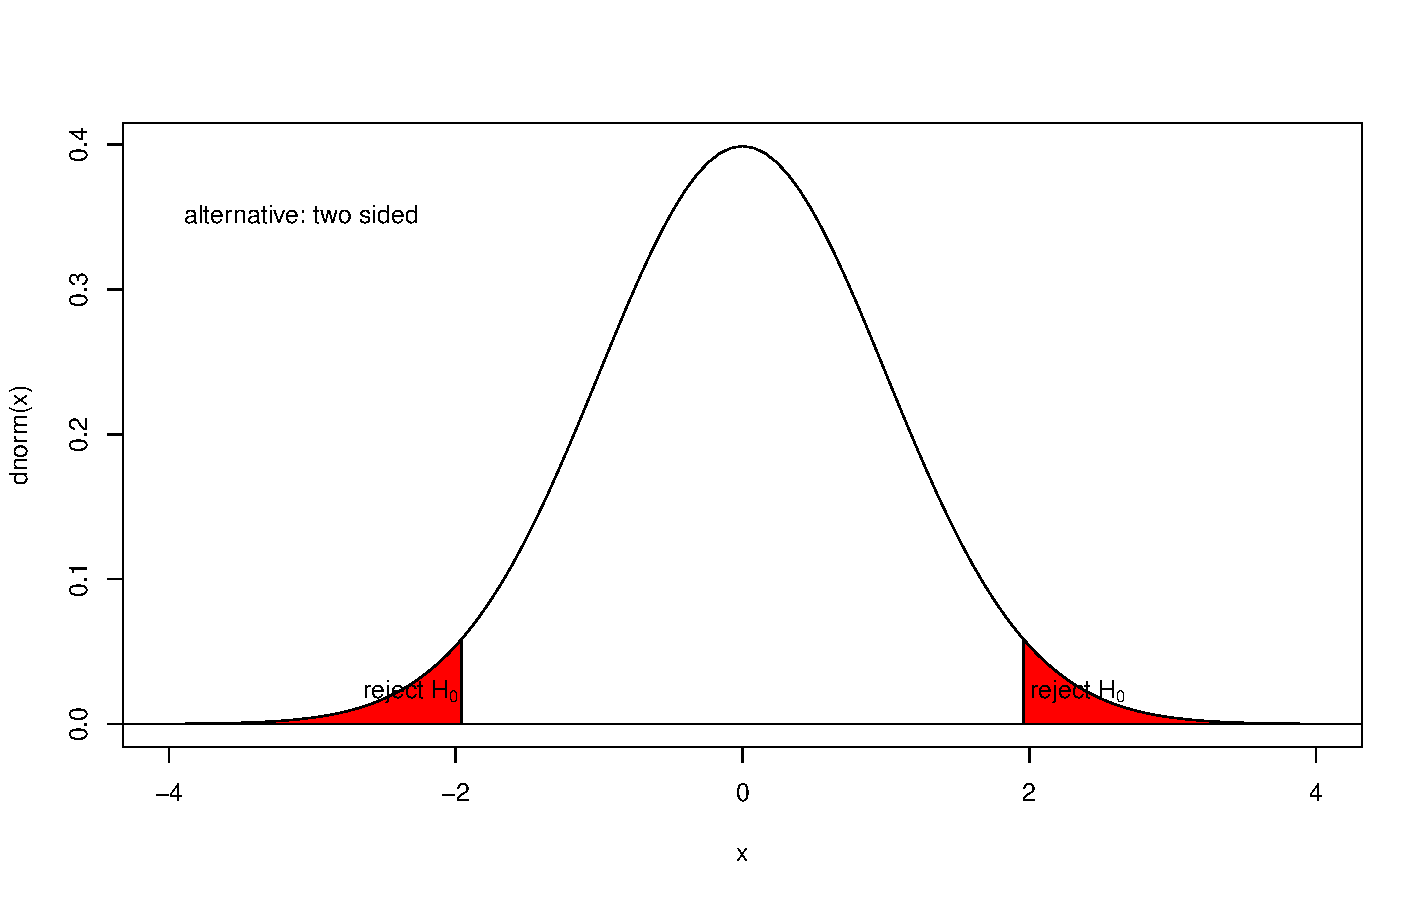
\includegraphics[width=11cm, height=7cm]{twosided.pdf}}
    \only<2>{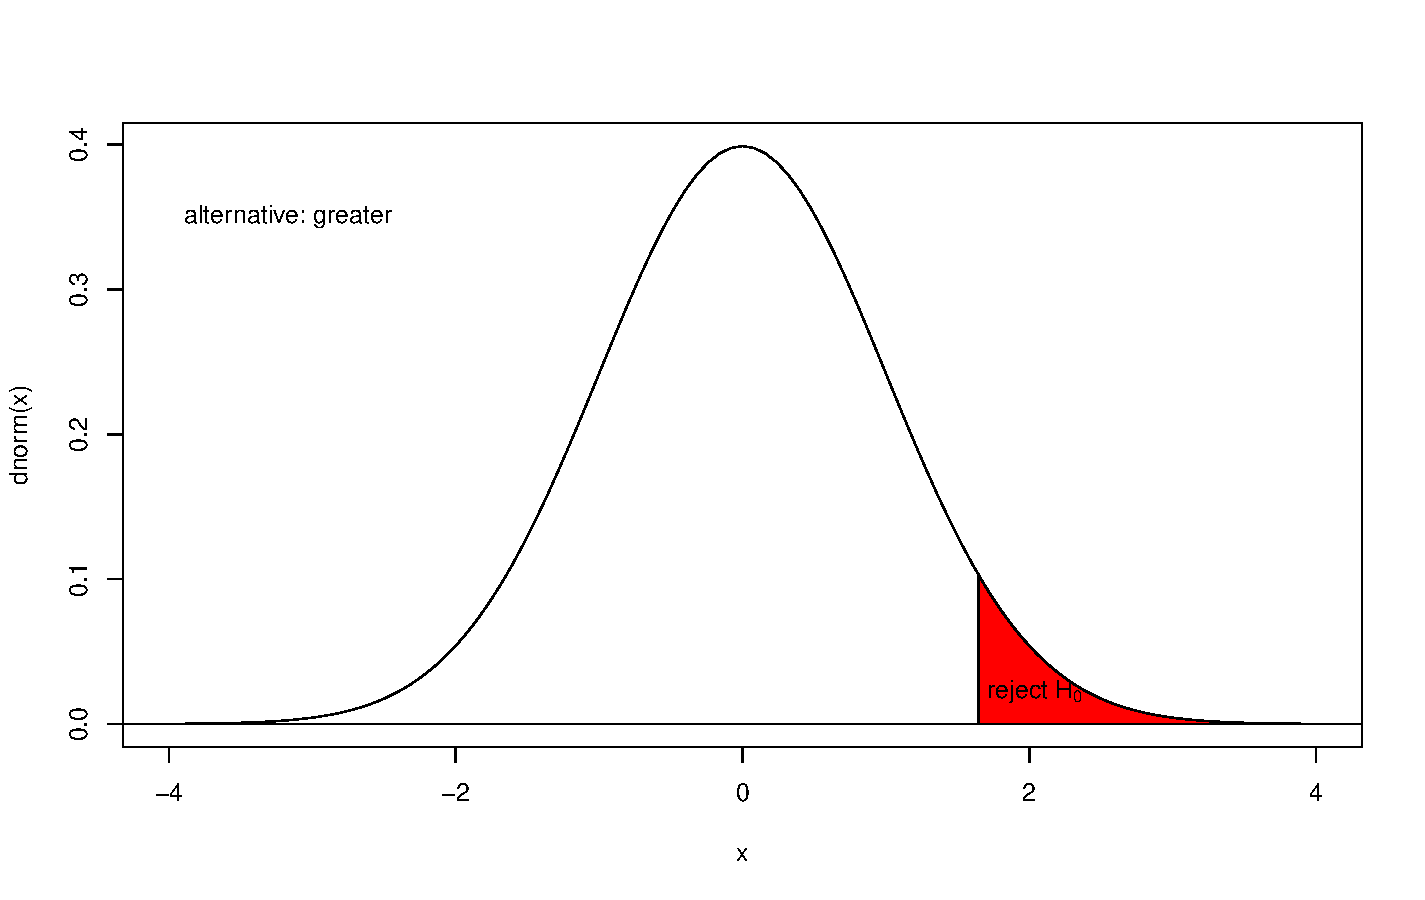
\includegraphics[width=11cm, height=7cm]{greater.pdf}}
    \only<3>{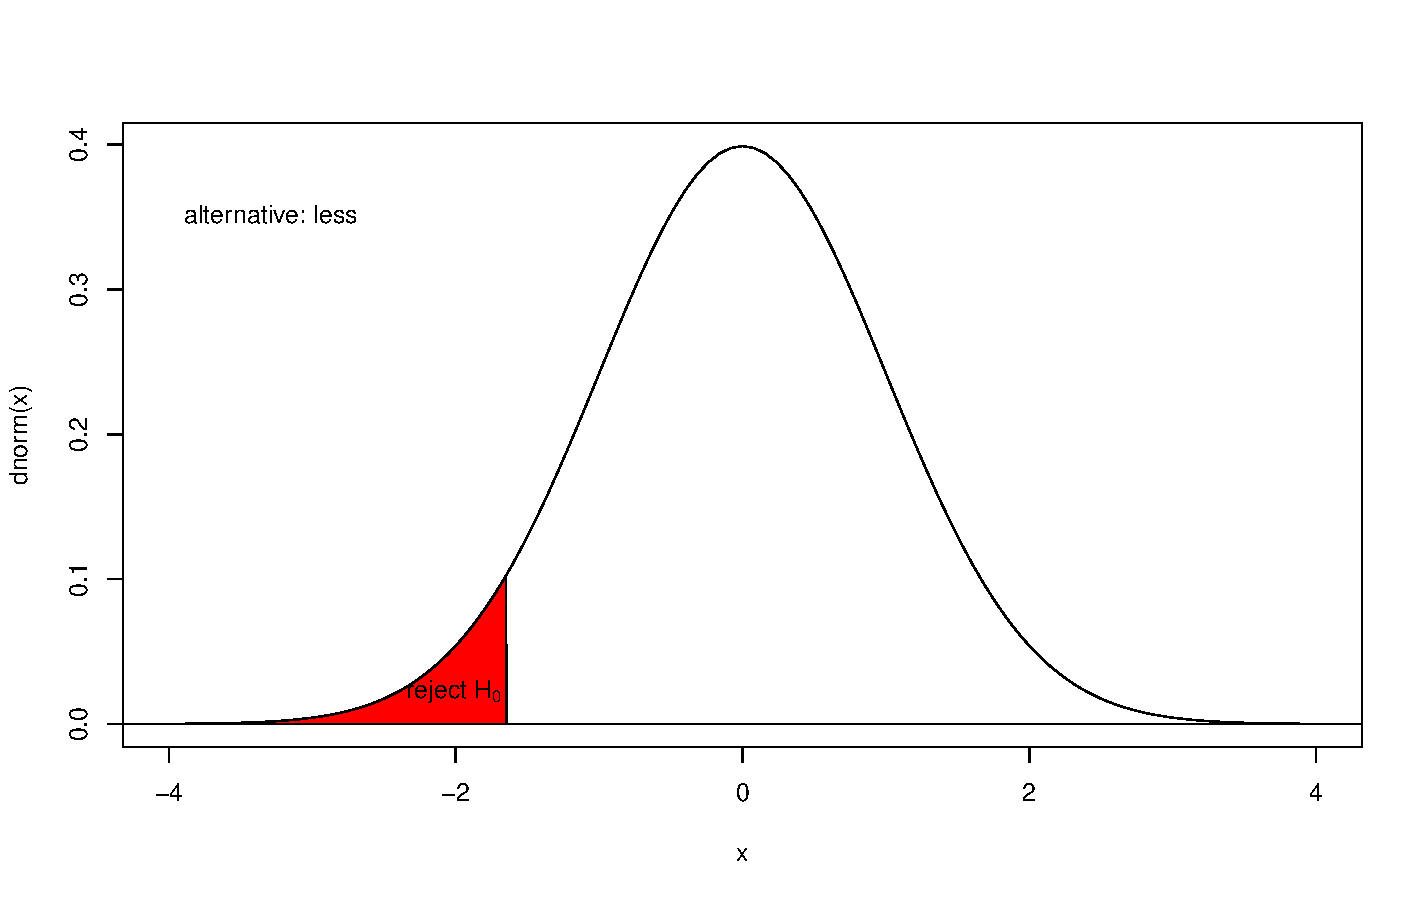
\includegraphics[width=11cm, height=7cm]{less.pdf}}
\end{frame}


\begin{frame}\frametitle{Alternatives}
  \begin{alertblock}{Note:}
    The p-value is the probability of the sample estimate (of the respective estimator) under the null.
  \end{alertblock}
\end{frame}

\section{Understand Hypothesis Tests}\small 
\subsection{Z-test}
\begin{frame}\frametitle{Z-test for a population mean} 
The z-test is a something like a t-test (it is like you would know almost everything about the perfect conditions. It uses the normal distribution as test statistic and is therefore a good example.
  \begin{block}{Objective}
    To investigate the significance of the difference between an assumed population mean $\mu_0$ and a sample mean $\bar{x}$.
  \end{block}
  \begin{alertblock}{Limitations}
    \begin{enumerate}
      \item It is necessary that the population variance $\sigma^2$ is known. 
      \item The test is accurate if the population is normally distributed. If the population is not normal, the test will still give an approximate guide.
    \end{enumerate}
  \end{alertblock}
\end{frame}


\begin{frame}[fragile]\frametitle{Z-test for a population mean}\footnotesize
    \begin{exampleblock}{Test statistic}
    $$Z = \frac{\bar{x}-\mu_0}{\sigma/\sqrt{n}}$$
  \end{exampleblock}
    \begin{enumerate}
    \item Write a function which takes a vector, the population standard deviation and the population mean as arguments and which gives the Z score as result. 
      \begin{itemize}
      \item name the function \texttt{ztest} or \texttt{my.z.test} - not \texttt{z.test} because \texttt{z.test} is already used
      \item set a default value for the population mean
      \end{itemize}
    \item add a line to your function that allows you to process numeric vectors containing missing values!
    \item the function \texttt{pnorm(Z)} gives the probability of $x \leq Z $. Change your function so that it has the p-value (for a two sided test) as result. 
    \item now let the result be a named vector containing the estimated difference, Z, p and the n.
    \end{enumerate}
You can always test your function using simulated values: \texttt{rnorm(100,mean=0)} gives you a vector containing 100 normal distributed values with mean 0.
\end{frame}

\begin{frame}[fragile]\frametitle{Z-test for a population mean}
Write a function which takes a vector, the population standard deviation and the population mean as arguments and which gives the Z score as result.
\begin{verbatim}
> ztest <- function(x,x.sd,mu=0){
+     sqrt(length(x)) * (mean(x)-mu)/x.sd
+ }
> set.seed(1)
> ztest(rnorm(100),x.sd = 1)
[1] 1.088874
\end{verbatim}
\end{frame}

\begin{frame}[fragile]\frametitle{Z-test for a population mean}
Add a line to your function that allows you to also process numeric vectors containing missing values!
\begin{verbatim}
> ztest <- function(x,x.sd,mu=0){
+     x <- x[!is.na(x)]
+     if(length(x) < 3) stop("too few values in x")
+     sqrt(length(x)) * (mean(x)-mu)/x.sd
+ }
\end{verbatim}
\end{frame}

\begin{frame}[fragile]\frametitle{Z-test for a population mean}
The function \texttt{pnorm(Z)} gives the probability of $x \leq Z $. Change your function so that it has the p-value (for a two sided test) as result. 
\begin{verbatim}
> ztest <- function(x,x.sd,mu=0){
+     x <- x[!is.na(x)]
+     if(length(x) < 3) stop("too few values in x")
+     z <- sqrt(length(x)) * (mean(x)-mu)/x.sd
+     2*pnorm(-abs(z))
+ }
> set.seed(1)
> ztest(rnorm(100),x.sd = 1)
[1] 0.2762096
\end{verbatim}
\end{frame}


\begin{frame}[fragile]\frametitle{Z-test for a population mean}
Now let the result be a named vector containing the estimated difference, Z, p and the n.
\footnotesize
\begin{verbatim}
> ztest <- function(x,x.sd,mu=0){
+     x <- x[!is.na(x)]
+     if(length(x) < 3) stop("too few values in x")
+     est.diff <- mean(x)-mu
+     z <- sqrt(length(x)) * (est.diff)/x.sd
+     round(c(diff=est.diff,Z=z,pval=2*pnorm(-abs(z)),n=length(x)),4)
+ }
> set.seed(1)
> ztest(rnorm(100),x.sd = 1)
    diff        Z     pval        n 
  0.1089   1.0889   0.2762 100.0000 

\end{verbatim}
\end{frame}

\begin{frame}\frametitle{Z-test for a population mean} 
  \begin{block}{Variants}
    \begin{enumerate}
      \item Z-test for two population means (variances known and equal)
      \item Z-test for two population means (variances known and unequal)
    \end{enumerate}
    To investigate the statistical significance of the difference between an assumed population mean $\mu_0$ and a sample mean $\bar{x}$. There is a function \texttt{z.test()} in the \texttt{BSDA} package.
  \end{block}
  \begin{alertblock}{Limitations (again)}
    \begin{enumerate}
      \item It is necessary that the population variance $\sigma^2$ is known. 
      \item The test is accurate if the population is normally distributed. If the population is not normal, the test will still give an approximate guide.
    \end{enumerate}
  \end{alertblock}
\end{frame}

\subsection{Simulation Exercises}
\begin{frame}\frametitle{Simulation Exercises} 
  \begin{enumerate}
  \item Now sample 100 values from a Normal distribution with mean 10 and standard deviation 2 and use a z-test to compare it against the population mean 10. What is the p-value?
  \item Now do the sampling and the testing 1000 times, what would be the number of statistically significant results? Use \texttt{replicate()} (which is a wrapper of \texttt{tapply()}) or a \texttt{for()} loop! Record at least the p-values and the estimated differences! Use \texttt{table()} to count the p-vals below 0.05. What type of error do you associate with it? What is the smallest absolute difference with a p-value below 0.05?
  \item Repeat the simulation above, change the sample size to 1000 in each of the 1000 samples! How many p-values below 0.05? What is now the smallest absolute difference with a p-value below 0.05?
  \end{enumerate}
\end{frame}


\begin{frame}[fragile]\frametitle{Simulation Exercises -- Solutions} 
  \begin{itemize}
  \item Now sample 100 values from a Normal distribution with mean 10 and standard deviation 2 and use a z-test to compare it against the population mean 10. What is the p-value? What the estimated difference?
  \end{itemize}
\begin{verbatim}
> ztest(rnorm(100,mean=10,sd=2),x.sd=2,mu=10)["pval"]
  pval 
0.0441   
> ztest(rnorm(100,mean=10,sd=2),x.sd=2,mu=10)["diff"]
   diff 
-0.0655 
> ztest(rnorm(100,mean=10,sd=2),x.sd=2,mu=10)[c("pval","diff")]
  pval   diff 
0.4515 0.1506 
\end{verbatim}
\end{frame}


\begin{frame}[fragile]\frametitle{Simulation Exercises -- Solutions} 
  \begin{itemize}
  \item Now do the sampling and the testing 1000 times, what would be the number of statistically significant results? Use \texttt{replicate()} (which is a wrapper of \texttt{tapply()}) or a \texttt{for()} loop. Record at least the p-values and the estimated differences! Transform the result into a data frame.
  \end{itemize}
using \texttt{replicate()}\footnotesize
\begin{verbatim}
> res <- replicate(1000, ztest(rnorm(100,mean=10,sd=2),x.sd=2,mu=10))
> res <- as.data.frame(t(res))
> head(res)
     diff       Z   pval   n
1 -0.2834 -1.4170 0.1565 100
2  0.2540  1.2698 0.2042 100
3 -0.1915 -0.9576 0.3383 100
4  0.1462  0.7312 0.4646 100
5  0.1122  0.5612 0.5747 100
6 -0.0141 -0.0706 0.9437 100
\end{verbatim}
\end{frame}


\begin{frame}[fragile]\frametitle{Simulation Exercises -- Solutions} 
  \begin{itemize}
  \item Now do the sampling and the testing 1000 times, what would be the number of statistically significant results? Use \texttt{replicate()} (which is a wrapper of \texttt{tapply()}) or a \texttt{for()} loop. Record at least the p-values and the estimated differences! Transform the result into a data frame.
  \end{itemize}
using \texttt{replicate()} II\footnotesize
\begin{verbatim}
> res <- replicate(1000, ztest(rnorm(100,mean=10,sd=2),x.sd=2,mu=10),
+                        simplify = F)
> res <- as.data.frame(Reduce(rbind,res))
> head(res)
        diff       Z   pval   n
init -0.0175 -0.0874 0.9304 100
     -0.0751 -0.3757 0.7072 100
.1    0.0446  0.2232 0.8234 100
.2   -0.3642 -1.8209 0.0686 100
.3   -0.2039 -1.0195 0.3080 100
.4   -0.1872 -0.9359 0.3493 100
\end{verbatim}
\end{frame}



\begin{frame}[fragile]\frametitle{Simulation Exercises -- Solutions} 
  \begin{itemize}
  \item Now do the sampling and the testing 1000 times, what would be the number of statistically significant results? Use \texttt{replicate()} (which is a wrapper of \texttt{tapply()}) or a \texttt{for()} loop. Record at least the p-values and the estimated differences! Transform the result into a data frame.
  \end{itemize}
using \texttt{for()} \scriptsize
\begin{verbatim}
> res <- matrix(numeric(2000),ncol=2)
> for(i in seq.int(1000)){
+     res[i,] <- ztest(rnorm(100,mean=10,sd=2),x.sd=2,mu=10)[c("pval","diff")] }
> res <- as.data.frame(res)
> names(res) <- c("pval","diff")
> head(res)
    pval    diff
1 0.0591 -0.3775
2 0.2466  0.2317
3 0.6368  0.0944
4 0.5538 -0.1184
5 0.9897 -0.0026
6 0.7748  0.0572
\end{verbatim}
\end{frame}

\begin{frame}[fragile]\frametitle{Simulation Exercises -- Solutions} 
\begin{itemize}
\item Use \texttt{table()} to count the p-vals below 0.05. What type of error do you associate with it? What is the smallest absolute difference with a p-value below 0.05?
\end{itemize}\footnotesize
\begin{verbatim}
> table(res$pval < 0.05)

FALSE  TRUE 
  960    40 
> tapply(abs(res$diff),res$pval < 0.05,summary)
$`FALSE`
   Min. 1st Qu.  Median    Mean 3rd Qu.    Max. 
 0.0002  0.0585  0.1280  0.1411  0.2068  0.3847 

$`TRUE`
   Min. 1st Qu.  Median    Mean 3rd Qu.    Max. 
 0.3928  0.4247  0.4408  0.4694  0.5102  0.6859 

> min(abs(res$diff[res$pval<0.05]))
[1] 0.3928
\end{verbatim}
\end{frame}

\begin{frame}[fragile]\frametitle{Simulation Exercises -- Solutions} 
\begin{itemize}
\item Repeat the simulation above, change the sample size to 1000 in each of the 1000 samples! How many p-values below 0.05? What is now the smallest absolute difference with a p-value below 0.05?
\end{itemize}\small
\begin{verbatim}
> res2 <- replicate(1000, ztest(rnorm(1000,mean=10,sd=2),
+                              x.sd=2,mu=10))
> res2 <- as.data.frame(t(res2))
> head(res2)
     diff       Z   pval    n
1 -0.0731 -1.1559 0.2477 1000
2  0.0018  0.0292 0.9767 1000
3  0.0072  0.1144 0.9089 1000
4 -0.1145 -1.8100 0.0703 1000
5 -0.1719 -2.7183 0.0066 1000
6  0.0880  1.3916 0.1640 1000
\end{verbatim}
\end{frame}


\begin{frame}[fragile]\frametitle{Simulation Exercises -- Solutions} 
\begin{itemize}
\item Repeat the simulation above, change the sample size to 1000 in each of the 1000 samples! How many p-values below 0.05? What is now the smallest absolute difference with a p-value below 0.05?
\end{itemize}\small
\begin{verbatim}
> table(res2$pval < 0.05)

FALSE  TRUE 
  946    54 
> tapply(abs(res2$diff),res$pval < 0.05,summary)
$`FALSE`
   Min. 1st Qu.  Median    Mean 3rd Qu.    Max. 
0.00010 0.02092 0.04285 0.05149 0.07400 0.22610 

$`TRUE`
   Min. 1st Qu.  Median    Mean 3rd Qu.    Max. 
0.00240 0.02115 0.04535 0.05435 0.08433 0.14760 
\end{verbatim}
\end{frame}

\begin{frame}\frametitle{Simulation Exercises Part II} 
  \begin{enumerate}
  \item Concatenate the both resulting data frames from above using \texttt{rbind()}
  \item Plot the distributions of the pvals and the difference per sample size. Use \texttt{ggplot2} with an appropriate geom (density/histogram)
  \item What is the message?
  \end{enumerate}
\end{frame}

\begin{frame}[fragile]\frametitle{Simulation Exercises -- Solutions} 
\begin{itemize}
\item Concatenate the both resulting data frames from above using \texttt{rbind()}
\item Plot the distributions of the pvals and the difference per sample size. Use \texttt{ggplot2} with an appropriate geom (density/histogram)
\end{itemize}\small
\begin{verbatim}
> res <- rbind(res,res2)  
> require(ggplot2)
> ggplot(res,aes(x=pval)) +
+     geom_histogram(bin=0.1,fill="forestgreen") +
+     facet_grid(~ n)
> ggsave("hist.png")
\end{verbatim}
\end{frame}

\begin{frame}[fragile]\frametitle{Simulation Exercises -- Solutions} 
\begin{center}
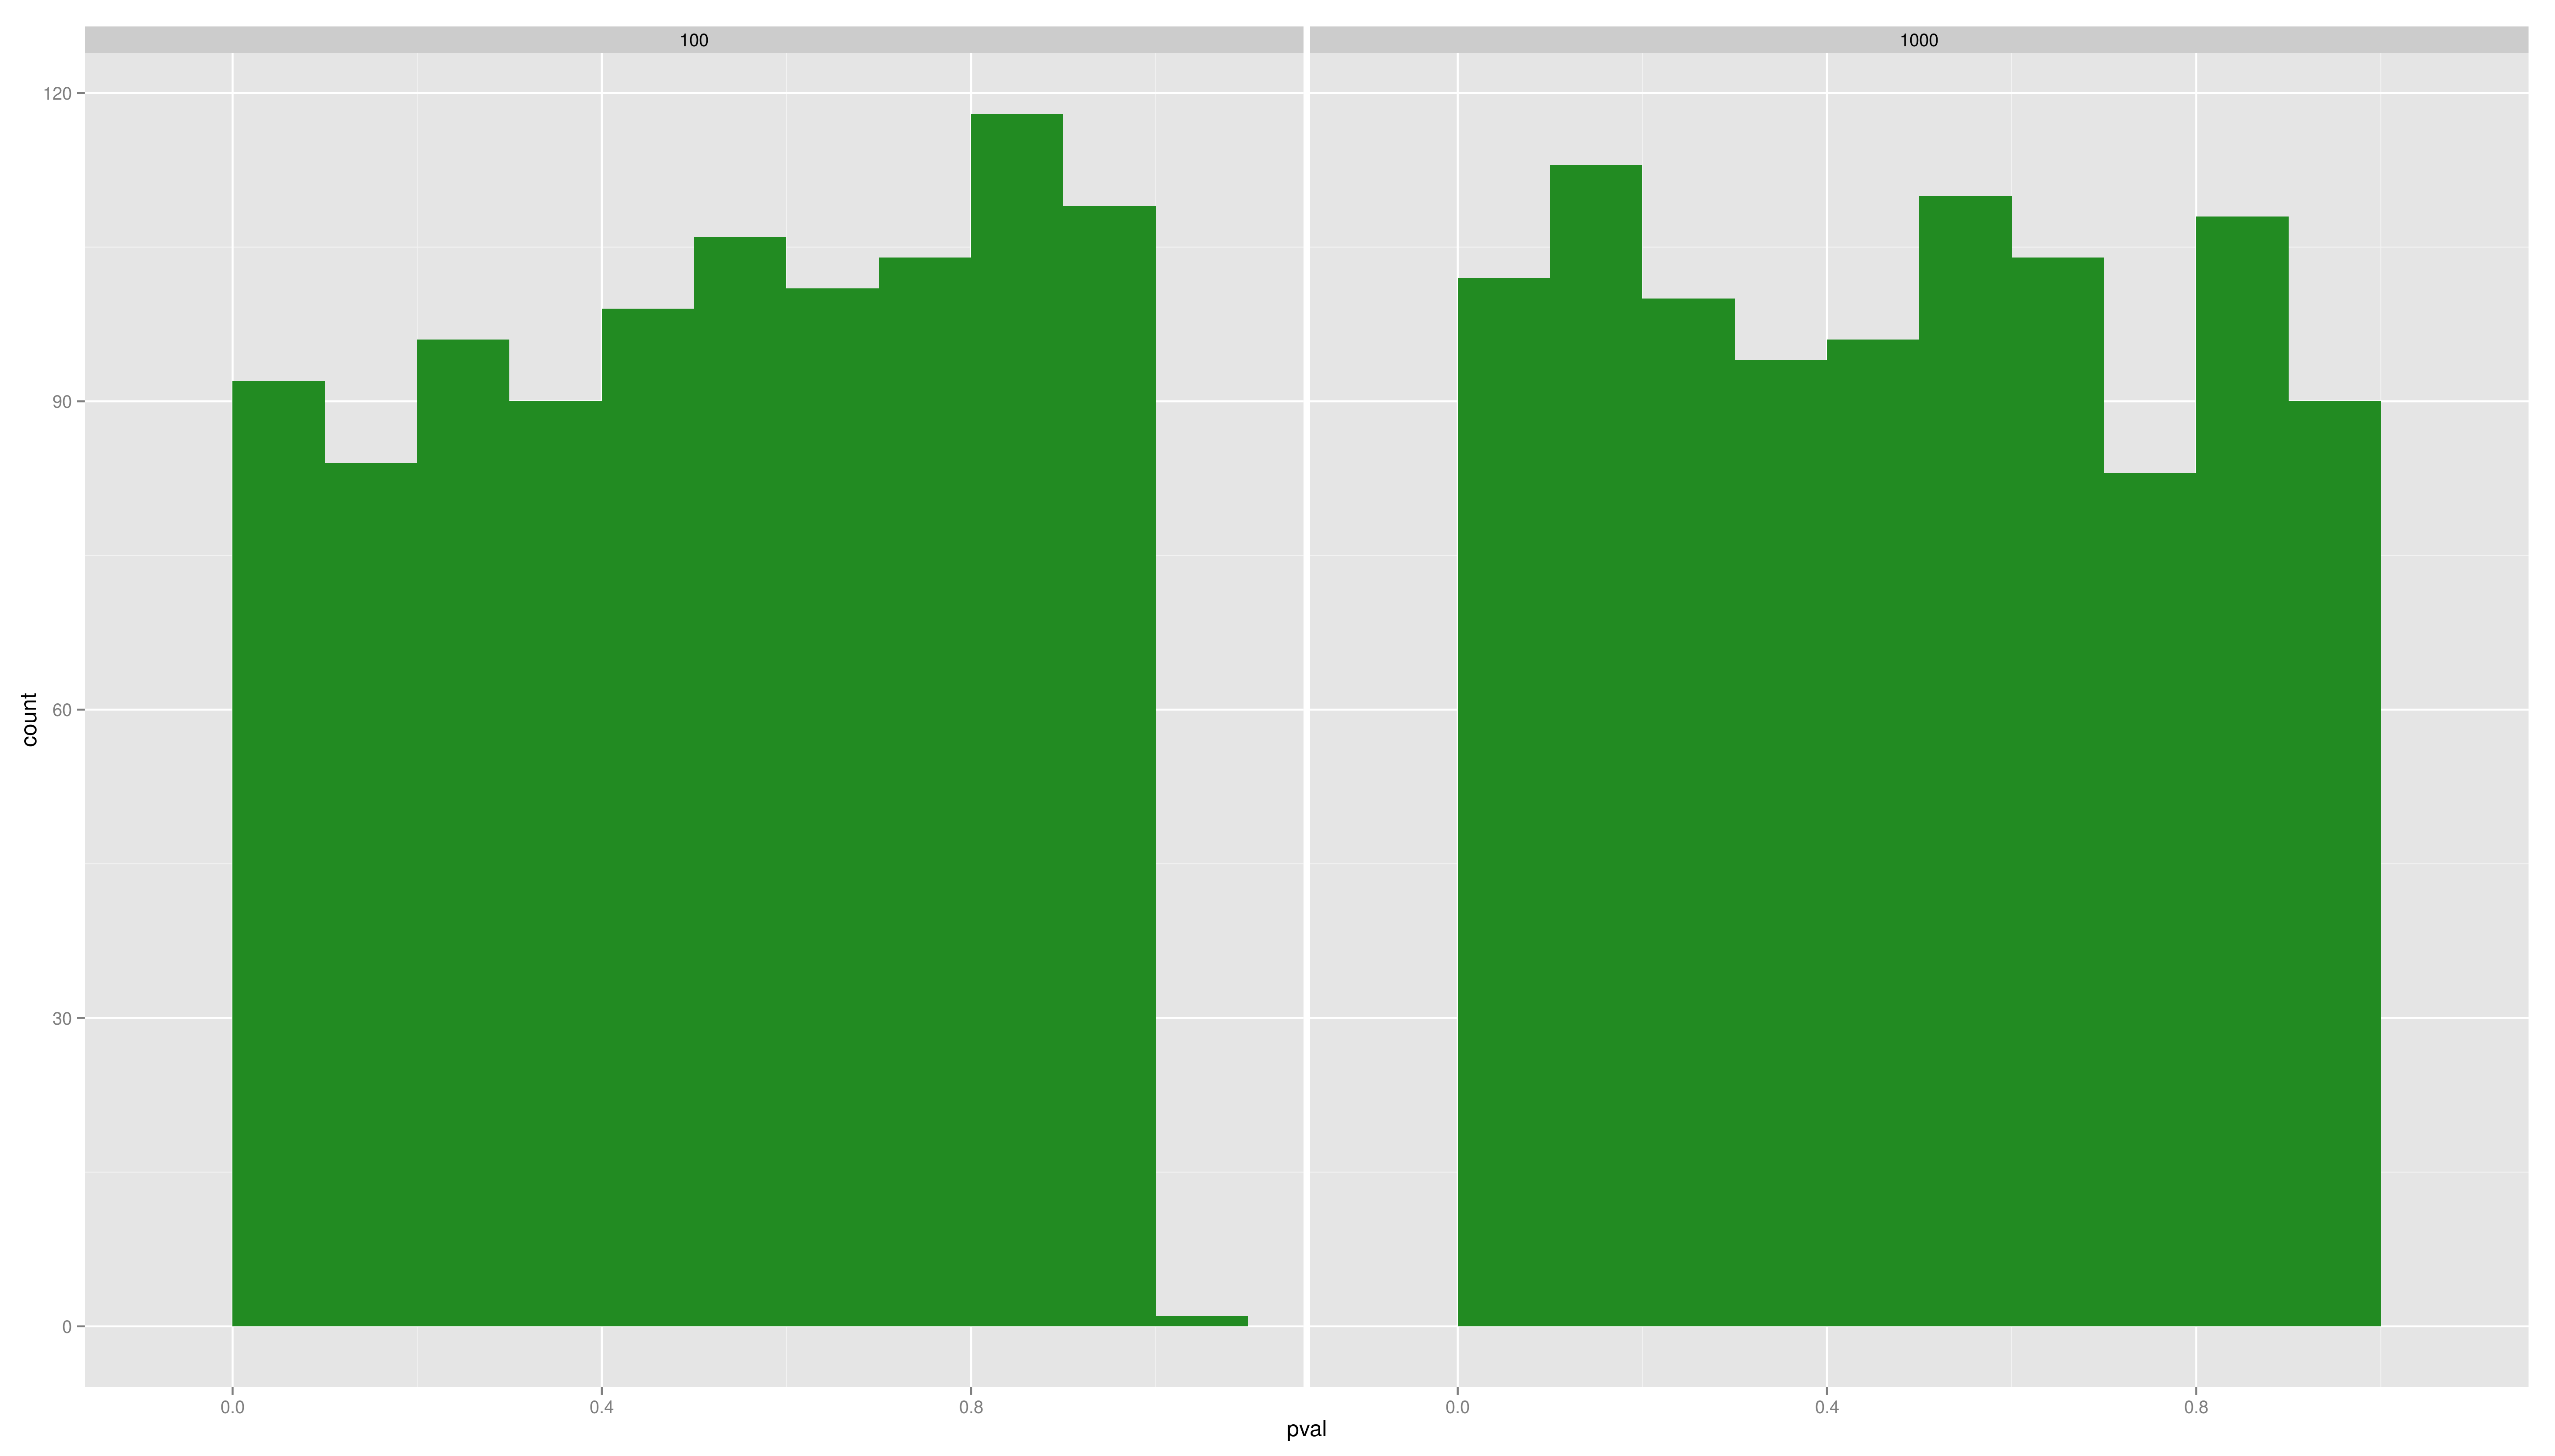
\includegraphics[width=8cm,height=6cm]{hist.png}
\end{center}
\end{frame}

\begin{frame}[fragile]\frametitle{Simulation Exercises -- Solutions} 
\begin{itemize}
\item Plot the distributions of the pvals and the difference per sample size. Use \texttt{ggplot2} with an appropriate geom (density/histogram)
\end{itemize}\small
\begin{verbatim}
> ggplot(res,aes(x=diff,colour=factor(n))) +
+     geom_density(size=3)
> ggsave("dens.png")
\end{verbatim}
\end{frame}

\begin{frame}[fragile]\frametitle{Simulation Exercises -- Solutions} 
\begin{center}
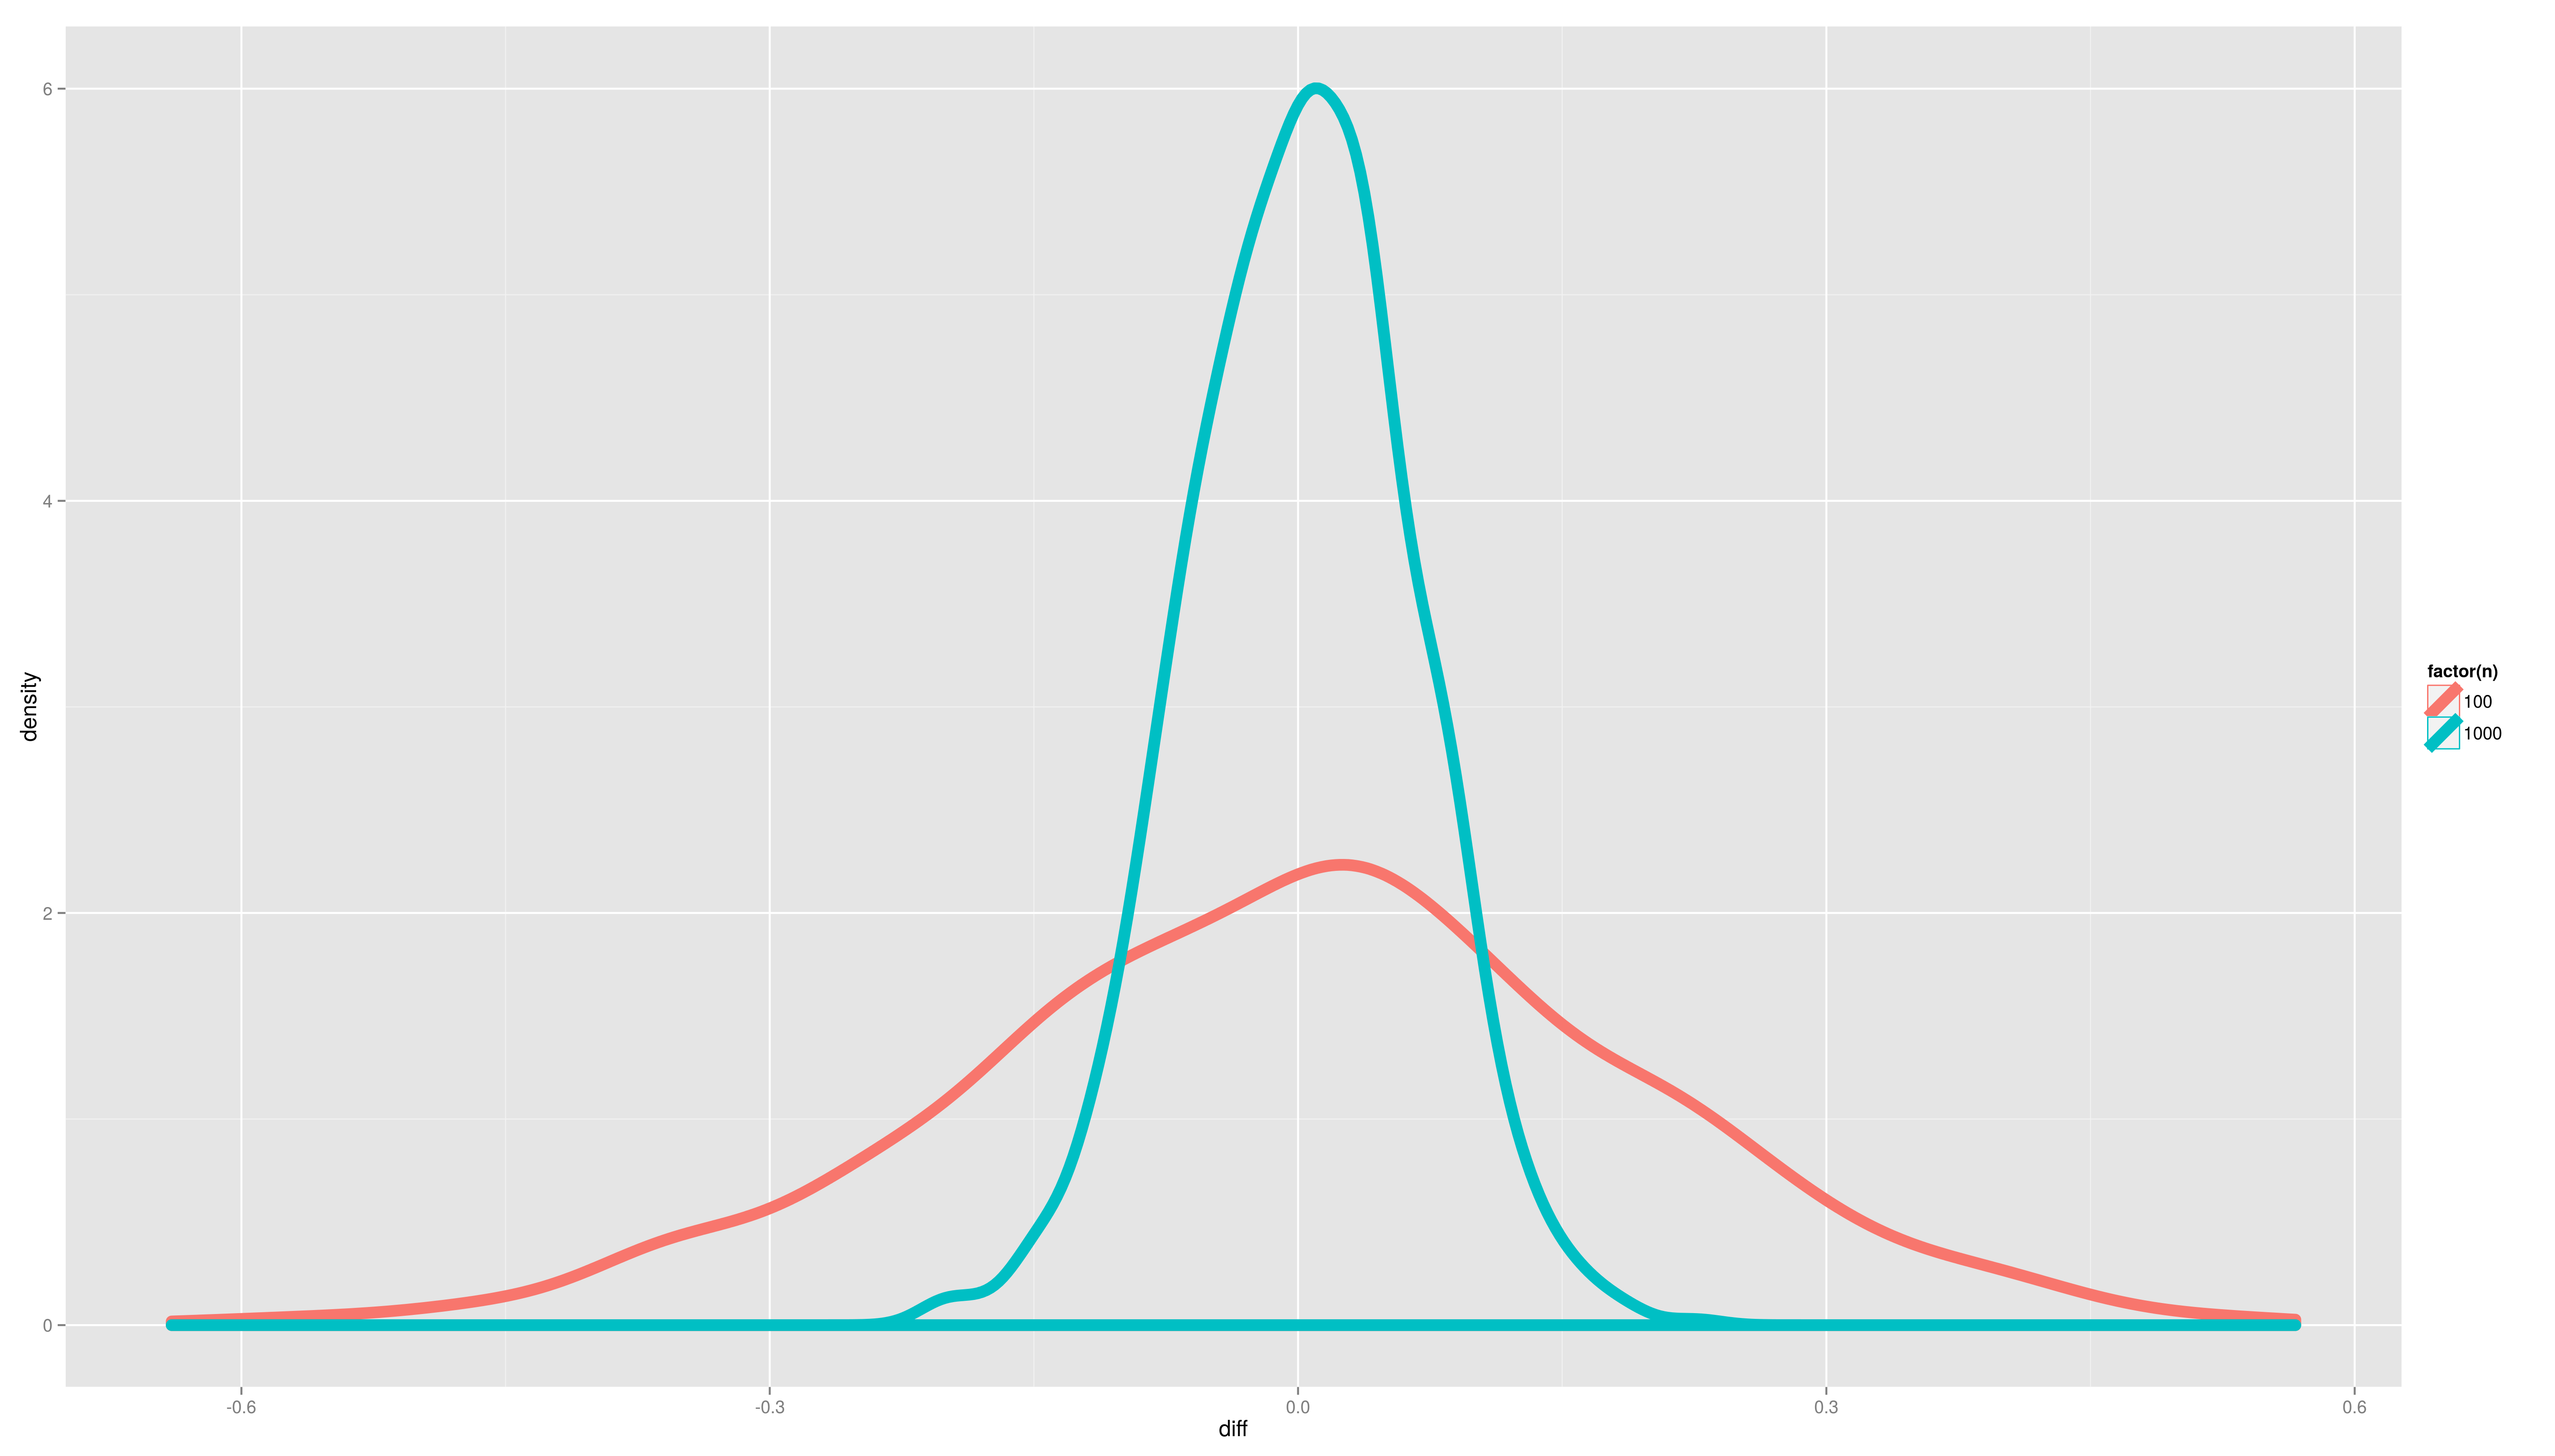
\includegraphics[width=8cm,height=6cm]{dens.png}
\end{center}
\end{frame}


\begin{frame}[fragile]\frametitle{Simulation Exercises -- Solutions} 
\begin{center}
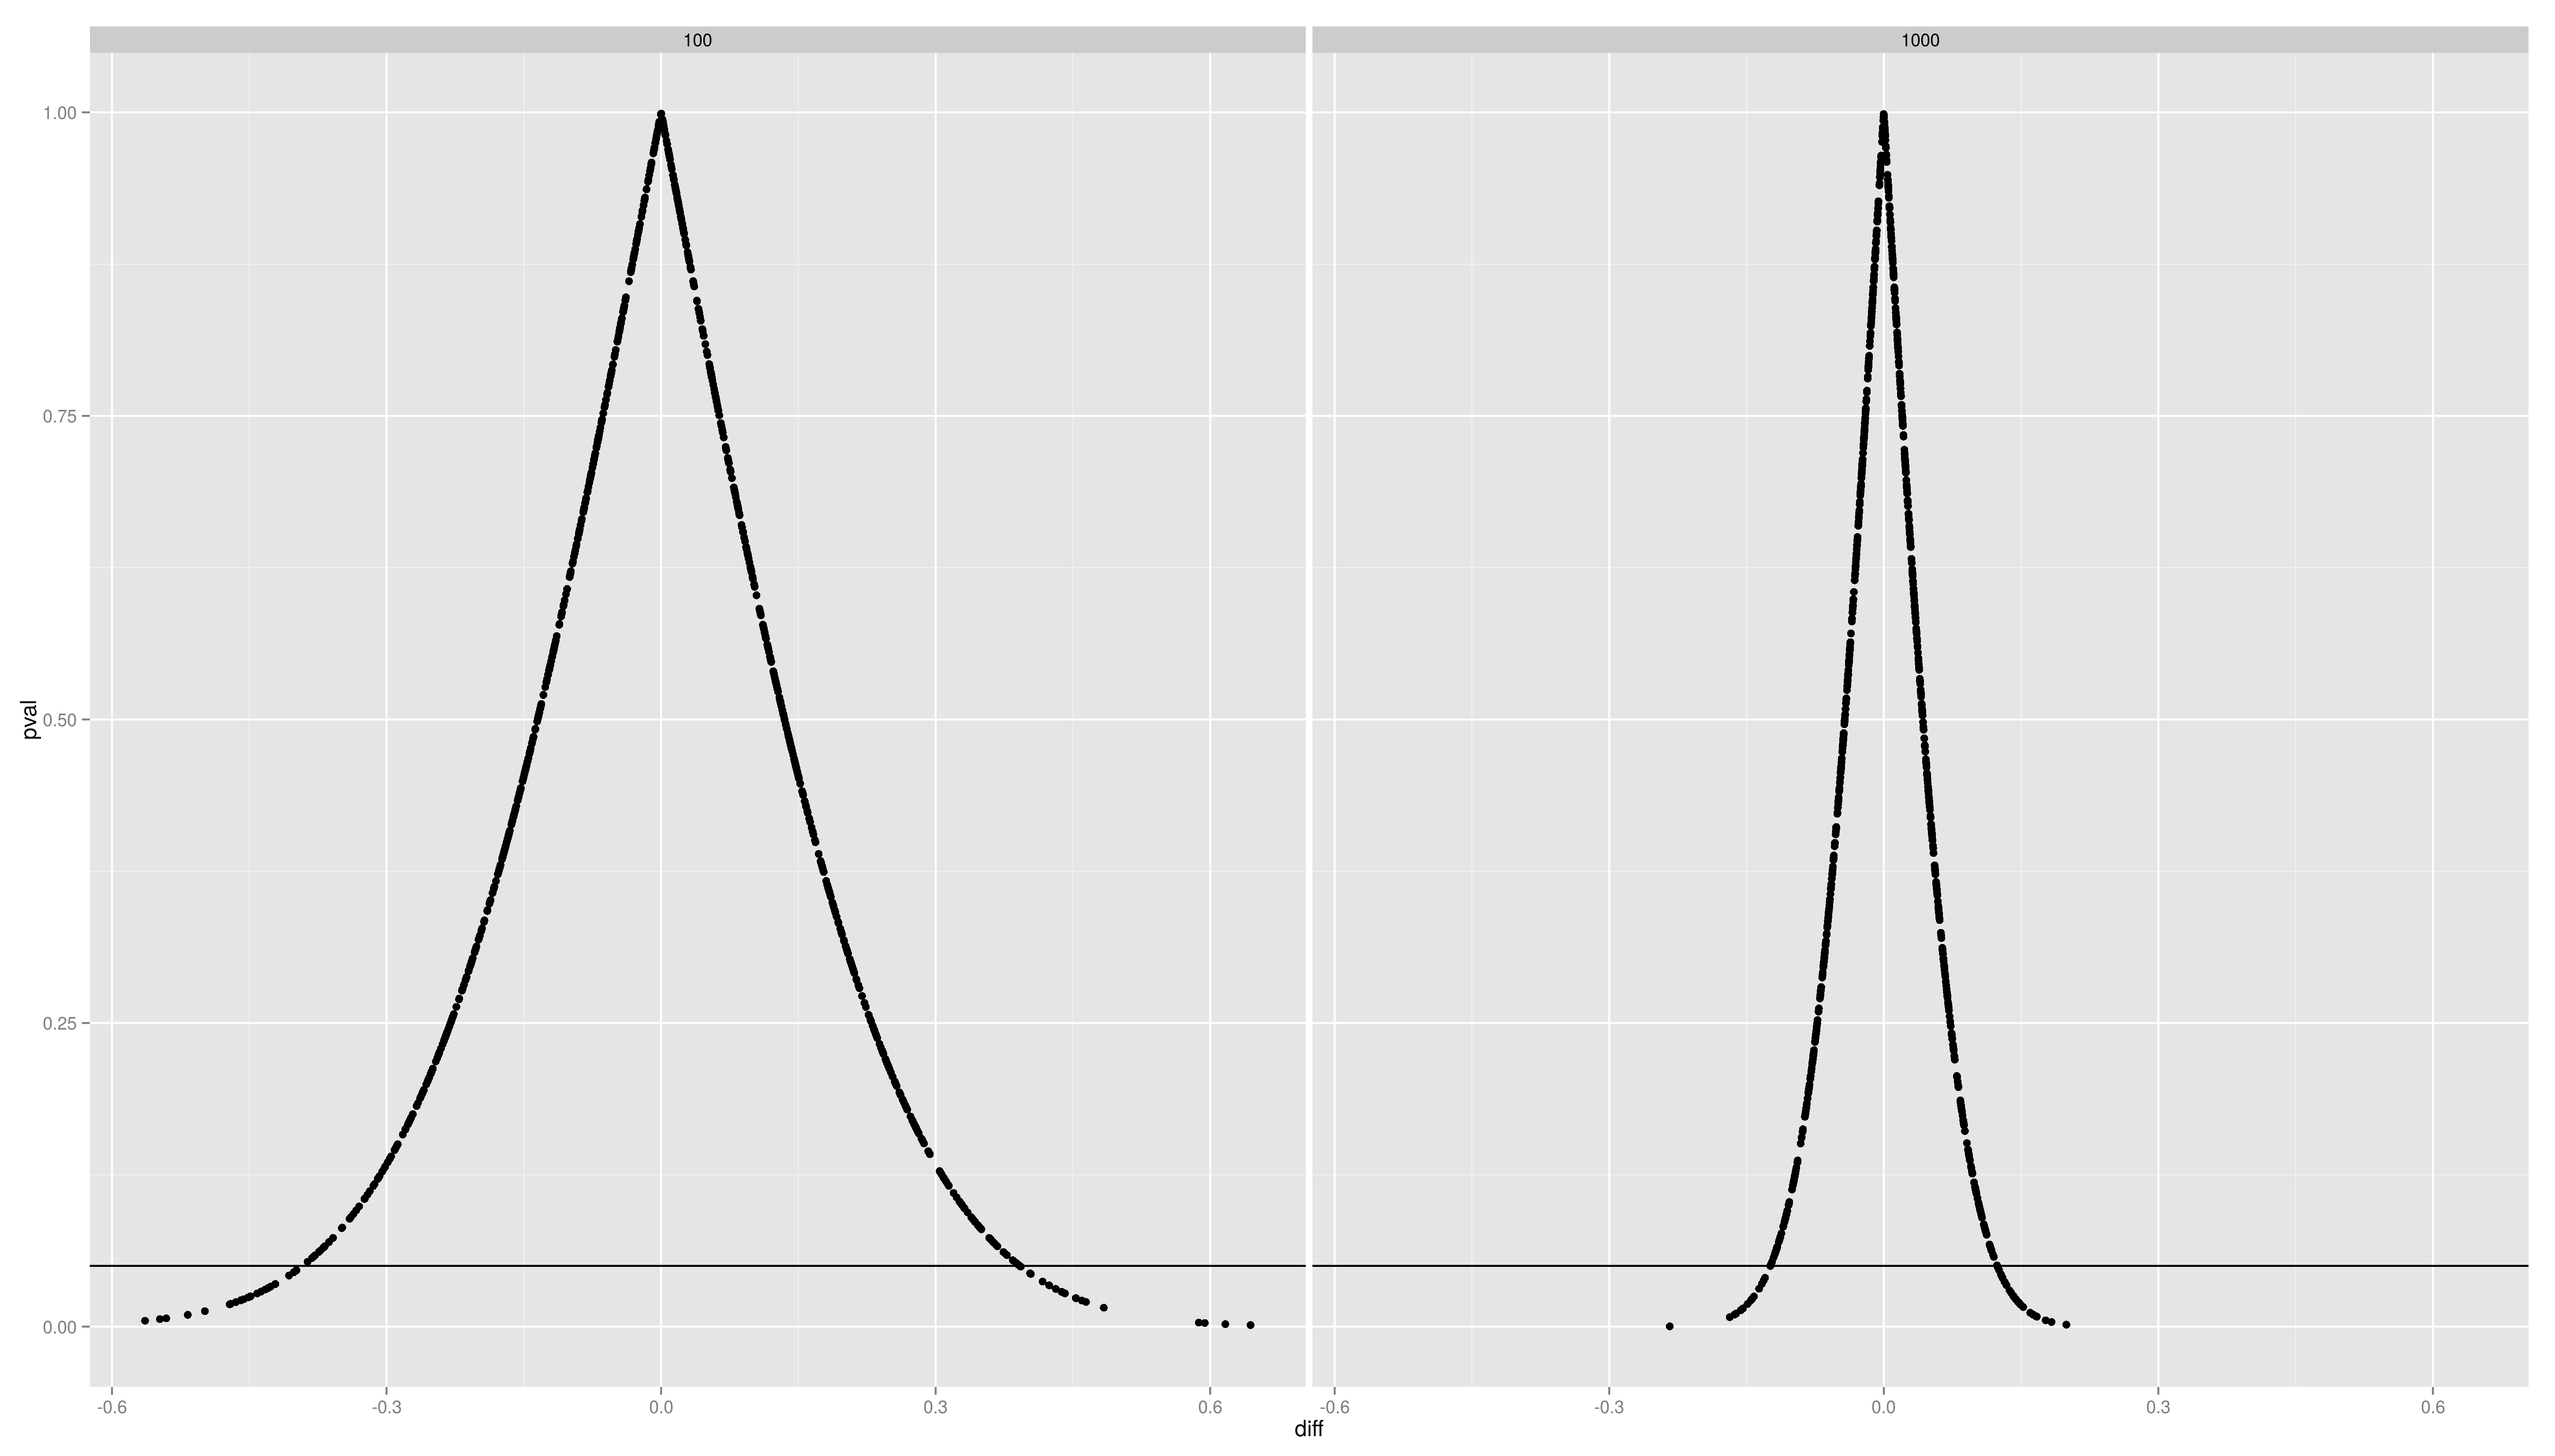
\includegraphics[width=8cm,height=6cm]{point.png}
\end{center}
\end{frame}

\begin{frame}[fragile]\frametitle{Simulation Exercises -- Solutions} 
\begin{center}
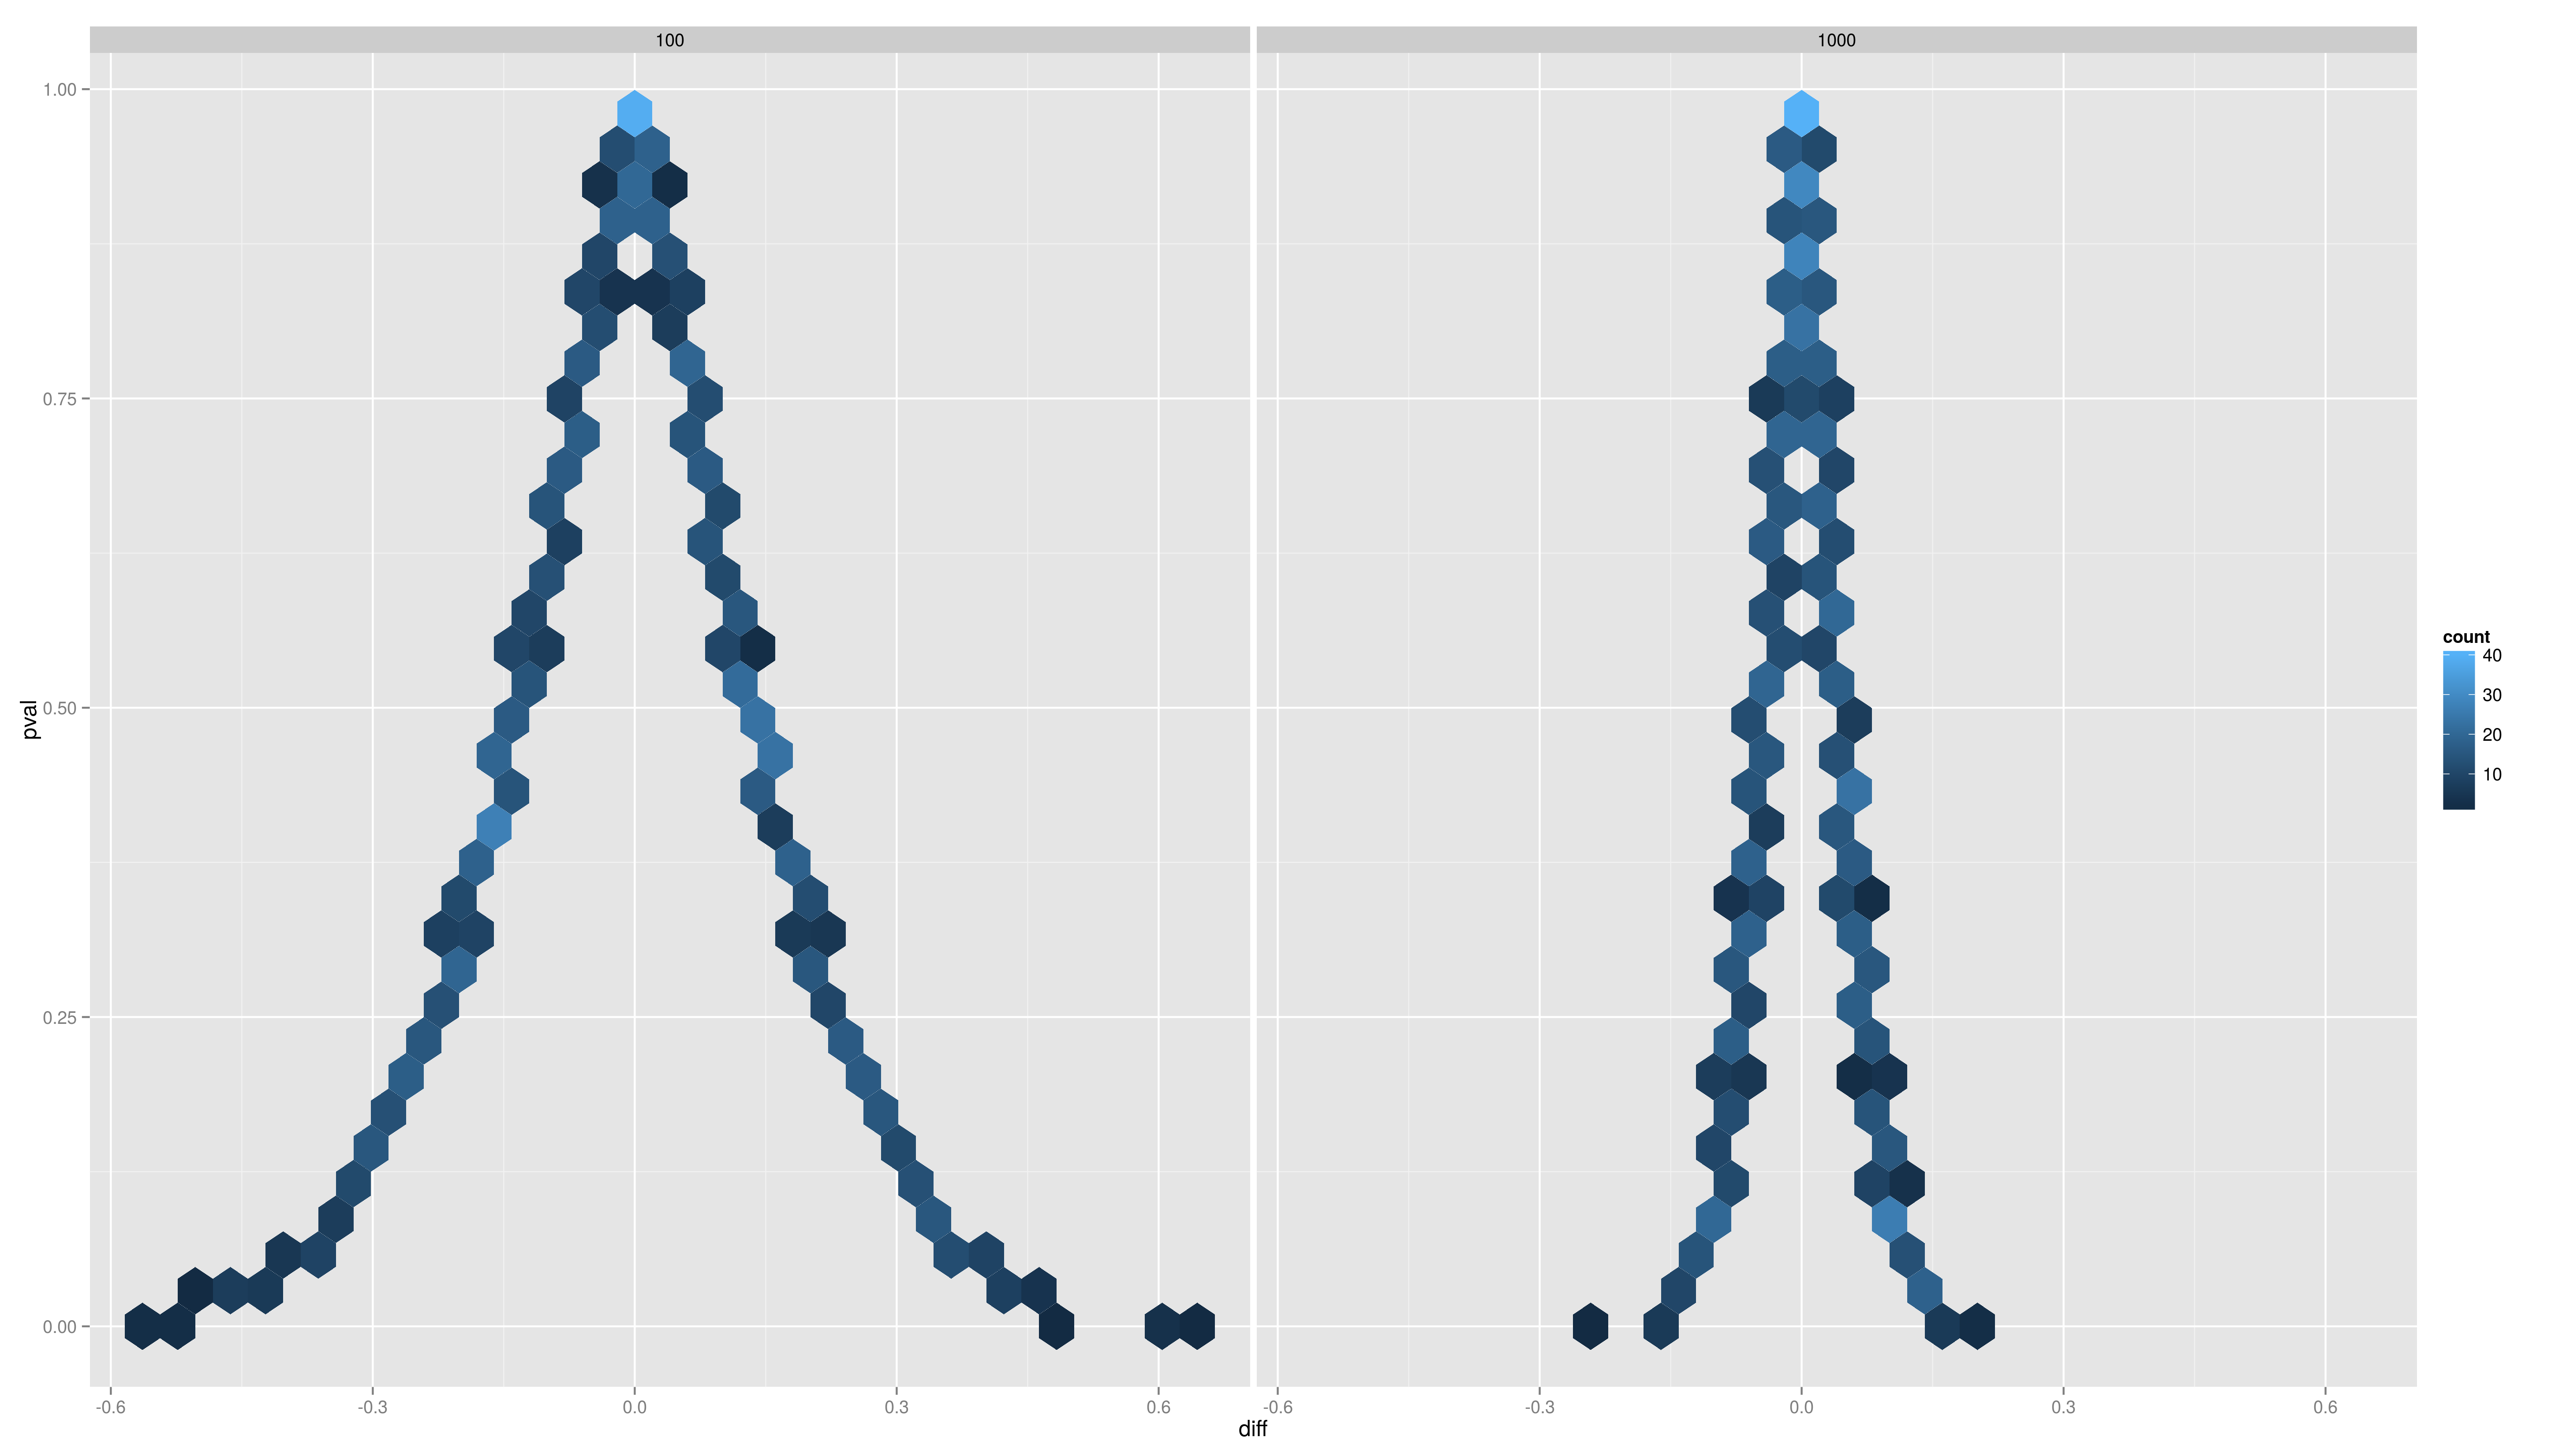
\includegraphics[width=8cm,height=6cm]{dens2d.png}
\end{center}
\end{frame}


\section{t-Tests}
\subsection{One Sample t-test}
\defverbatim{\ttesta}{
\begin{verbatim}
> set.seed(1)
> x <- rnorm(12)
> t.test(x,mu=0) ## population mean 0

	One Sample t-test

data:  x
t = 1.1478, df = 11, p-value = 0.2754
alternative hypothesis: true mean is not equal to 0
95 percent confidence interval:
 -0.2464740  0.7837494
sample estimates:
mean of x 
0.2686377 
\end{verbatim}
}


\defverbatim{\ttestb}{
\begin{verbatim}


> t.test(x,mu=1) ## population mean 1

	One Sample t-test

data:  x
t = -3.125, df = 11, p-value = 0.009664
alternative hypothesis: true mean is not equal to 1
95 percent confidence interval:
 -0.2464740  0.7837494
sample estimates:
mean of x 
0.2686377 
\end{verbatim}
}

\begin{frame}[fragile]\frametitle{t-tests}
A t-test is any statistical hypothesis test in which the test statistic follows a \emph{Student's t distribution} if the null hypothesis is supported.
\begin{itemize}
\item \emph{one sample t-test}: test a sample mean against a population mean
$$ t = \frac{\bar{x}-\mu_0}{s/\sqrt{n}}$$ where $\bar{x}$ is the sample mean, $s$ is the sample standard deviation and $n$ is the sample size. The degrees of freedom used in this test is $n-1$
\end{itemize}
\end{frame}

\begin{frame}[fragile]\frametitle{One Sample t-test}
\only<1>{\ttesta}
\only<2>{\ttestb}
\end{frame}


\subsection{Two Sample t-tests}

\defverbatim{\ttestc}{

}

\begin{frame}[fragile]\frametitle{Two Sample t-tests}
There are two ways to perform a two sample t-test in R:
\begin{itemize}
\item given two vectors \texttt{x} and \texttt{y} containing the measurement values from the respective groups \texttt{t.test(x,y)}
\item given one vector \texttt{x} containing all the measurement values and one vector \texttt{g} containing the group membership $t.test(x \sim g)$ (read: x dependend on g)
\end{itemize}
\end{frame}

\begin{frame}[fragile]\frametitle{Two Sample t-tests: two vector syntax}\footnotesize
\begin{verbatim}
> set.seed(1)
> x <- rnorm(12)
> y <- rnorm(12)
> g <- sample(c("A","B"),12,replace = T)
> t.test(x,y)

	Welch Two Sample t-test

data:  x and y
t = 0.5939, df = 20.012, p-value = 0.5592
alternative hypothesis: true difference in means is not equal to 0
95 percent confidence interval:
 -0.5966988  1.0717822
sample estimates:
 mean of x  mean of y 
0.26863768 0.03109602   
\end{verbatim}
\end{frame}


\begin{frame}[fragile]\frametitle{Two Sample t-tests: formula syntax}\footnotesize
\begin{verbatim}




> t.test(x ~ g)

	Welch Two Sample t-test

data:  x by g
t = -0.6644, df = 6.352, p-value = 0.5298
alternative hypothesis: true difference in means is not equal to 0
95 percent confidence interval:
 -1.6136329  0.9171702
sample estimates:
mean in group A mean in group B 
      0.1235413       0.4717726 
\end{verbatim}
\end{frame}


\begin{frame}[fragile]\frametitle{Welch/Satterthwaite vs. Student}
  \begin{itemize}
  \item if not stated otherwise \texttt{t.test()} will not assume that the variances in the both groups are equal
  \item if one knows that both populations have the same variance set the \texttt{var.equal} argument to TRUE to perform a student's t-test
  \end{itemize}
\end{frame}

\begin{frame}[fragile]\frametitle{Student's t-test}\footnotesize
\begin{verbatim}



> t.test(x, y, var.equal = T)

	Two Sample t-test

data:  x and y
t = 0.5939, df = 22, p-value = 0.5586
alternative hypothesis: true difference in means is not equal to 0
95 percent confidence interval:
 -0.5918964  1.0669797
sample estimates:
 mean of x  mean of y 
0.26863768 0.03109602   
\end{verbatim}
\end{frame}

\begin{frame}[fragile]\frametitle{t-test}
  \begin{itemize}
  \item the t-test, especially the Welch test is appropriate whenever the values are normally distributed
  \item it is also recommended for group sizes $\geq 30$ (robust against deviation from normality)
  \end{itemize}
\end{frame}

\begin{frame}[fragile,allowframebreaks]\frametitle{Exercises} 
  \begin{enumerate}
  \item use a t-test to compare \texttt{TTime} according to \texttt{Stim.Type}, visualize it. What is the problem?
  \item now do the same for Subject 1 on pre and post test (use \texttt{filter()} or indexing to get the resp. subsets)
  \item use the following code to do the test on every subset \texttt{Subject} and \texttt{testid}, try to figure what is happening in each step:\tiny
\begin{verbatim}
data.l <- split(data,list(data$Subject,data$testid),drop=T)
tmp.l <- lapply(data.l,function(x) {
    if(min(table(x$Stim.Type)) < 5) return(NULL)
    tob <- t.test(x$TTime ~ x$Stim.Type)
    tmp <- data.frame(
        Subject = unique(x$Subject),
        testid = unique(x$testid),
        mean.group.1 = tob$estimate[1],
        mean.group.2 = tob$estimate[2],
        name.test.stat = tob$statistic,
        conf.lower = tob$conf.int[1],
        conf.upper = tob$conf.int[2],
        pval = tob$p.value,
        alternative = tob$alternative,
        tob$method)})
res <- Reduce(rbind,tmp.l)
\end{verbatim}\normalsize
  \item make plots to visualize the results. 
  \item how many tests have a statistically significant result? How many did you expect? Is there a tendency? What could be the next step?
  \end{enumerate}
\end{frame}

\begin{frame}[fragile]\frametitle{Exercises - Solutions}
  \begin{itemize}
  \item use a t-test to compare \texttt{TTime} according to \texttt{Stim.Type}, visualize it. What is the problem?
  \end{itemize}\tiny
\begin{verbatim}
> t.test(data$TTime ~ data$Stim.Type)

	Welch Two Sample t-test

data:  data$TTime by data$Stim.Type
t = -6.3567, df = 9541.891, p-value = 2.156e-10
alternative hypothesis: true difference in means is not equal to 0
95 percent confidence interval:
 -2773.574 -1466.161
sample estimates:
      mean in group hit mean in group incorrect 
               17579.77                19699.64   
> ggplot(data,aes(x=Stim.Type,y=TTime)) +
+     geom_boxplot()
\end{verbatim}
\end{frame}


\begin{frame}[fragile,allowframebreaks]\frametitle{Exercises - Solutions}
  \begin{itemize}
  \item now do the same for Subject 1 on pre and post test (use \texttt{filter()} or indexing to get the resp. subsets)
  \end{itemize}\footnotesize
\begin{verbatim}
> t.test(data$TTime[data$Subject==1 & data$testid=="test1"] ~
+        data$Stim.Type[data$Subject==1 & data$testid=="test1"])

	Welch Two Sample t-test

data:  data$TTime[data$Subject == 1 & data$testid == "test1"] by data$Stim.Type[data$Subject == 1 & data$testid == "test1"]
t = -0.5846, df = 44.183, p-value = 0.5618
alternative hypothesis: true difference in means is not equal to 0
95 percent confidence interval:
 -4930.842  2713.191
sample estimates:
      mean in group hit mean in group incorrect 
               8248.175                9357.000 

> t.test(data$TTime[data$Subject==1 & data$testid=="test2"] ~
+        data$Stim.Type[data$Subject==1 & data$testid=="test2"])

	Welch Two Sample t-test

data:  data$TTime[data$Subject == 1 & data$testid == "test2"] by data$Stim.Type[data$Subject == 1 & data$testid == "test2"]
t = -1.7694, df = 47.022, p-value = 0.08332
alternative hypothesis: true difference in means is not equal to 0
95 percent confidence interval:
 -7004.4904   448.9388
sample estimates:
      mean in group hit mean in group incorrect 
               4012.480                7290.256 

\end{verbatim}
\end{frame}

\begin{frame}[fragile]\frametitle{Exercises - Solutions}
  \begin{itemize}
  \item make plots to visualize the results
  \end{itemize}\footnotesize
\begin{verbatim}
> ggplot(data,aes(x=testid,y=TTime)) +
+    geom_boxplot(aes(fill=Stim.Type)) +
+    facet_wrap(~Subject)
> ggplot(data,aes(x=factor(Subject),y=TTime)) +
+    geom_boxplot(aes(fill=Stim.Type)) +
+    facet_wrap(~testid)
\end{verbatim}
\end{frame}


\begin{frame}[fragile]\frametitle{Exercises - Solutions}
  \begin{itemize}
  \item how many tests have an statistically significant result? How many did you expect? 
  \end{itemize}\footnotesize
\begin{verbatim}
> table(res$pval < 0.05)

FALSE  TRUE 
  165    22 
> prop.table(table(res$pval < 0.05))

    FALSE      TRUE 
0.8823529 0.1176471 
> 
\end{verbatim}
\end{frame}


\begin{frame}[fragile,allowframebreaks]\frametitle{Exercises - Solutions}
  \begin{itemize}
  \item  What could be the next step?
  \end{itemize}\tiny
\begin{verbatim}
tmp.l <- lapply(data.l,function(x) {
    if(min(table(x$Stim.Type)) < 5) return(NULL)
    tob <- t.test(x$TTime ~ x$Stim.Type)
    tmp <- data.frame(
        Subject = unique(x$Subject),
        testid = unique(x$testid),
        perc.corr = sum(x$Stim.Type=="hit")/sum(!is.na(x$Stim.Type)),
        mean.group.1 = tob$estimate[1],
        mean.group.2 = tob$estimate[2],
        name.test.stat = tob$statistic,
        conf.lower = tob$conf.int[1],
        conf.upper = tob$conf.int[2],
        pval = tob$p.value,
        alternative = tob$alternative,
        tob$method)})

res <- Reduce(rbind,tmp.l)

ggplot(res,aes(x=perc.corr,y=mean.group.1 - mean.group.2)) +
    geom_point() +
    geom_smooth()
\end{verbatim}
\end{frame}

\end{document}
